\chapter{Project schedule}

In this section, we will include the updated project schedule. We designed a Gantt Chart for the project schedule to maintain track of time. We couldn't create tasks that would indicate a slippage since it would disrupt the critical path. However, the Gantt Chart does not consider Saturdays and Sundays as working days, as well as, a task cannot start on Saturdays or Sundays, so these two days can be labeled as a slippage time. We must allow slippage time, due to other university's homework, exams, or even illness.

In Figure \ref{fig:gantt_chart}, we can see the tasks on the left and their visualizations on the right, along with the highlighted critical path. We split the project into 3 Sprints, as we are utilizing the scrum methodology. The only differences between the old and new Gantt Charts are that we changed and corrected Sprint 2 tasks, as well as added new Sprint 3 tasks and that we changed the dependency of some tasks from Finish-Start to Start-Start, as it didn't make any sense for some tasks to wait for a specific task to finish, because we could work simultaneously. Furthermore, for Sprint 2, we added the entire hardware delay (buying, delivery, and collection), which was not anticipated in the prior Gantt Chart. The tasks that will be included in the second Sprint are those stated in section \nameref{Future Work}.

The logic of each sprint is the same as it was before. That means that each sprint contains a sprint plan, the implementation/development, sprint Retrospective and a milestone signaling the Sprint's completion.


\afterpage{%
    \clearpage% Flush earlier floats (otherwise order might not be correct)
    \thispagestyle{empty}% empty page style (?)
    \begin{landscape}% Landscape page
        \centering % Center table

        \section{Gantt Chart}
          \begin{figure}[ht!]
            \centering % Center tables
            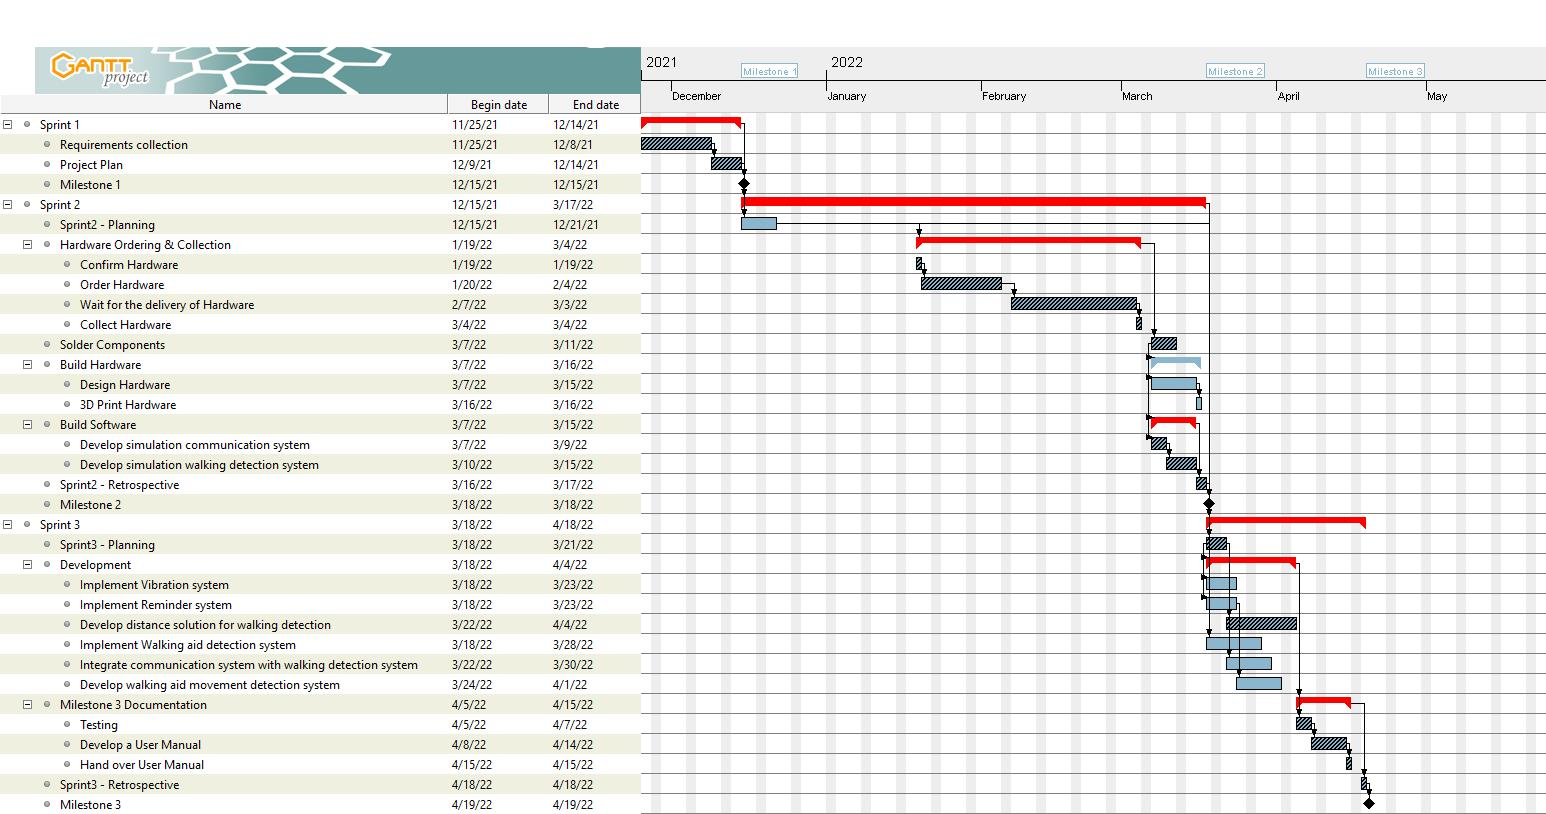
\includegraphics[width=1.8\textwidth,keepaspectratio]{./Images/Milestone2_Gantt_Chart.jpg}
            \caption{This is the updated Gantt Chart}
            \label{fig:gantt_chart}
          \end{figure}

        \pagebreak

    \end{landscape}
    \clearpage% Flush page
}
